\section{Persistenz}
Die Apps werden vom System beendet, ohne dass dies dem Benutzer bewusst ist. Das Sichern der Daten ist also Aufgabe der App. Es gibt zwei unterschiedliche Arten von Daten: Zustandsdaten der Views (aktuelle Eingabewerte, Checkboxes, etc.)  und Anwendungsdaten der Domain-Klassen.
\paragraph{View-Daten Persistieren} \code{onCreate} und \code{onSaveInstanceState} erhalten je ein Bundle Objekt, dies ist wie eine Map/Property List mit assoziierten String-Key Values. Mit einem Bundle kann man Daten wie beispielsweise eine eingegebene E-Mail Adresse zwischenspeichern.
\begin{lstlisting}[language=java]
public class MainActivity extends AppCompatActivity {
  @Override
  protected void onCreate(Bundle savedInstanceState) {
  super.onCreate(savedInstanceState);
  }
  @Override
  protected void onSaveInstanceState(Bundle outState) {
  super.onSaveInstanceState(outState);
  }
}
\end{lstlisting}
\textbf{Wichtig:} Der \code{super} Aufruf speichert alle Views die eine ID haben.\\
Die AppDaten sollten in \code{onPause} gesichert werden, da \code{onSaveInstanceState} nicht immer ausgeführt wird. 
Es gibt verschiedene Möglichkeiten um Daten zu sichern:
\begin{itemize}
\item \textbf{Shared Preferences:} Key-Value Paare für wenige Daten
\item \textbf{Files:} Für private Daten die mit anderen Programmen geteilt werden
\item \textbf{SQLite:} Für strukturierte Daten, die in einer relationalen Datenbank abgelegt werden können
\item \textbf{Cloud:} Nicht immer verfügbar, lokaler Zwischenspeicher nötig
\end{itemize}

\paragraph{View-Daten mit ViewModel}
Um Daten kurzfristig zu speichern(z.B Screen-Rotation). Daten werden nicht persistiert. Mehrere Activites oder Fragments können dieselbe ViewModel Instanz teilen.
\begin{lstlisting}[language=java]
public class MyViewModel extends ViewModel {
    private int currentSelection;
    public int getCurrentSelection() {
        return currentSelection;
    }
    public void setCurrentSelection(int currentSelection){
        this.currentSelection = currentSelection;
    }
}
// Verwendung
@Override
protected void onCreate(Bundle savedInstanceState){
    super.onCreate(savedInstanceState);
    setContentView(R.layout.activity_details);
    ...
    MyViewModel model = ViewModelProviders.of(this).get(MyViewModel.class);
    model.setCurrentSelection(0); 
}
\end{lstlisting}

\paragraph{Shared Preferences} Erlaubt sind Key-Value Paare mit Value vom Typ: \code{boolean | float | int | long| String | Set<String>}. 
\begin{lstlisting}[language=java]
SharedPreferences settings = getSharedPreferences(PREFS_NAME, MODE_PRIVATE);
SharedPreferences.Editor editor = settings.edit();
editor.putBoolean("disabled", false);
boolean isDisabled = settings.getBoolean("disabled", false);
// gibt false zurueck, falls key "disabled" nicht vorhanden
editor.commit();
\end{lstlisting}
Eine Art Observer für diese Settings ist der \code{settings. registerOnSharedPreferenceChangeListener}.
\paragraph{File Storage} Es gibt zwei Speicher-Typen in Android. Den internen (privaten) und den externen Speicher (extern muss nicht zwingend auf einem externen Medium liegen). In den internen Speicher schreibt man fast ganz normal, wie das in Java üblich ist.
\begin{lstlisting}[language=java]
FileOutputStream fos = openFileOutput(FILENAME, Context.MODE_PRIVATE);
fos.write("File content".getBytes());
fos.close();
\end{lstlisting}
Möchte man in den externen Speicher schreiben, um beispielsweise Daten anderen Apps zur verfügung zu stellen, braucht man zuerst die Permissions im Manifest zu setzten. 
\begin{lstlisting}[language=java]
File path = Environment.getExternalStoragePublicDirectory(Environment.DIRECTORY_PICTURES);
File file = new File(path, "HSR_Cat.png");
\end{lstlisting}
Es gibt Konstanten für verschiedene vordefinierte Verzeichnisse.
\paragraph{SQLite Storage} Der SQLite Storage eignet sich für relationale Daten wie Domain Objekte.
\begin{lstlisting}[language=java]
public class DBHelpter extends SQLiteOpenHelper {
  private static final int DATABASE_VERSION = 2;
  DBHelper(Context context) {
  super(context, DATABASE_NAME, null, DATABASE_VERSION);
  }
  @Override
  public void onCreate(SQLiteDatabase db) {
  db.execSQL("CREATE TABLE ....;");
  }
  @Override
  public void onUpgrade(SQLiteDatabase db, int oldVersion, int newVersion {}
}
// Irgendwo anders
DBHelper helper = new DBHelpber(this);
SQLiteDatabase db = helper.getReadableDatabase();
db.execSQL("SELECT * FROM ...";);
\end{lstlisting}

\section{Hintergrunddienste}
%TODO: Fix references
Da der Main-Thread für das GUI zuständig ist, und die Ereignisse in einer Queue abgearbeitet werden, sollte man keine lange andauernden Aufträge in diesem laufen lassen (Siehe \autoref{grundlagen:eventhandling} EventHandling).\\
Eine simple und schnelle Lösung ist die Verwendung von Java Threads. Dies ist in Ordnung für kleinere Aufgaben, welche das GUI nicht manipulieren. Möchte man das UI manipulieren muss man mit Hilfsmethoden wie \code{post()} arbeiten.
\begin{lstlisting}[language=java]
public void onClick(View v) {
  Runnable runnable = new Runnable() {
  @Override
  public void run() {
    final Bitmap bitmap = download("something");
    Runnable command = new Runnable() {
    @Override
    public void run() {
      imageView.setImageBitmap(bitmap);
    }
    };
    imageView.post(command); //command wird im UI-Thread ausgeführt
  }
  };
  Thread thread = new Thread(runnable);
  thread.start();
}
\end{lstlisting}
Mit \code{post()} übergibt man die \code{Runnable} Instanz dem UI-Thread und führt diesen aus. Das \code{command} wird also im UI-Thread ausgeführt.
\paragraph{AsyncTask} Typischerweise startet man eine Aufgabe die in einem eigenen Thread ablaufen soll, um am Ende wieder etwas auf den Main-Thread zu tun. Der AsyncTask nimmt Parameter als generische Typen entgegen, für die Aufgabe die man Durchführen will. Der \textbf{erste Parameter} ist der Typ des Inputs, der \textbf{zweite} der Typ des Feedbacks über den Fortschritt und der \textbf{dritte} der Typ des Outputs. Pre = Vor, Post = Nach
\begin{lstlisting}[language=java]
public class DownloadBitmapTask extends AsyncTask<String, Integer, Bitmap> {
  @Override
  protected void onPreExecute() {
  // UI-Thread
  super.onPreExecute();
  }
  @Override
  protected Bitmap doInBackground(String ... params) {
  // Eigener Thread
  publishProgress(10);
  return download(params[0]);
  }
  @Override
  protected void onPostExecute(Bitmap bitmap){
  //UI-Thread
  imageView.setImageBitmap(bitmap);
  }
  @Override
  protected void onProgressUpdate(Integer... values){
  //UI-Thread
  progressBar.setProgress(values[0]);
  }
}
\end{lstlisting}
Möchte man keine Information über den Fortschritt, setzt man den zweiten generischen Parameter auf \code{Void}.


\subsection{Layer Architecture}
\textbf{Presentation} \\
- Zuständig für Darstellung und Interaktion mit dem Benutzer \\
- Ist dadurch typischerweise sehr stark an UI-Toolkit gebunden \\
- Hat Zugriff auf Domain \\
\textbf{Domain} \\
- Businesslogik und Domainklassen ohne UI Funktionalität \\
- Wenig externe Abhängigkeiten, einfach zu testen \\
\textbf{Data} (auch Persistence, Datenhaltung)\\
- Implementiert die Speicherung der Daten, stellt diese Dienste der Domain zur Verfügung (z.B. DB, Cloud) \\
\textbf{Important:} Domain soll z.B nicht abhängig von Android werden, einfachere Testbarkeit. An den Schnittstellen der Layer wird gerne mit Interfaces und Fassaden gearbeitet um diese zu entkoppeln.

\paragraph{Observer Pattern}
Wird verwendet, dass man keine Zyklen hat.
\textbf{Zwei Rollen:} \\
- Subject welches beobachtet wird (z.B Model) \\
- Observer welcher beobachtet (z.B View) \\
- Observer meldet sich bei Subject an \\
- Subject meldet Änderungen \\
- Observer holt von Subject aktuellen Zustand \\
- Observer kennt Subject gut, Subject muss aber nichts über Observer wissen \\ 
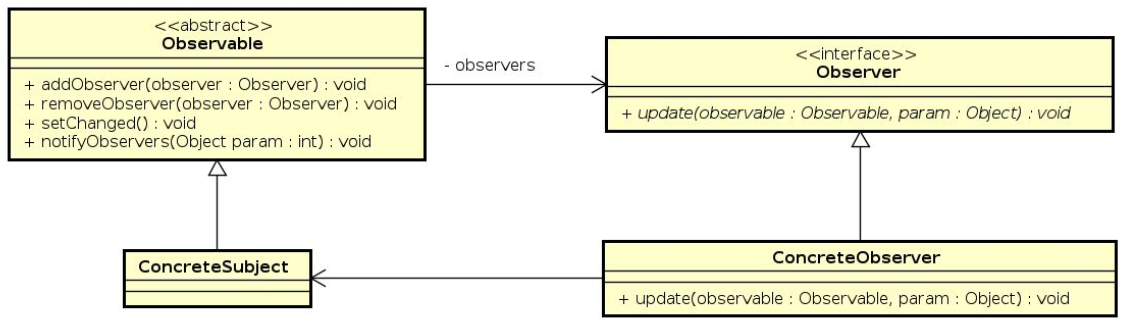
\includegraphics[scale=0.2]{img/observerpattern.png}

% TODO LiveData

\paragraph{Swipe-Refresh}
\begin{lstlisting}[language=xml]
<androidx.swiperefreshlayout.widget.SwipeRefreshLayout ...>
    <androidx.recyclerview.widget.RecyclerView .../>
</androidx.swiperefreshlayout.widget.SwipeRefreshLayout> 
\end{lstlisting}
\begin{lstlisting}[language=java]
final SwipeRefreshLayout swipeRefreshLayout = findViewById(R.id.swipeRefreshLayout);
swipeRefreshLayout.setOnRefreshListener(new SwipeRefreshLayout.OnRefreshListener() {
    @Override
    public void onRefresh() {
        adapter.refreshAll();
        swipeRefreshLayout.setRefreshing(false);
    } });
\end{lstlisting}

\paragraph{Model-View-Controller}
Android basiert lose auf dem MVC-Pattern. Controller durch Activity ersetzen: Activity manipuliert Model, Model list View und umgekehrt, View benachrichtigt Activity und Activity verändert View.

\paragraph{Model-View-Presenter}
Interfaces für View, Model (sogenannte Repositories) und Presenter. Fragen implementiert View-Interface. Fragment instanziert Presenter, verbindet Presenter mit Repository-Model und View (sich selbst).






\subsection{Komponenten einer Android App}
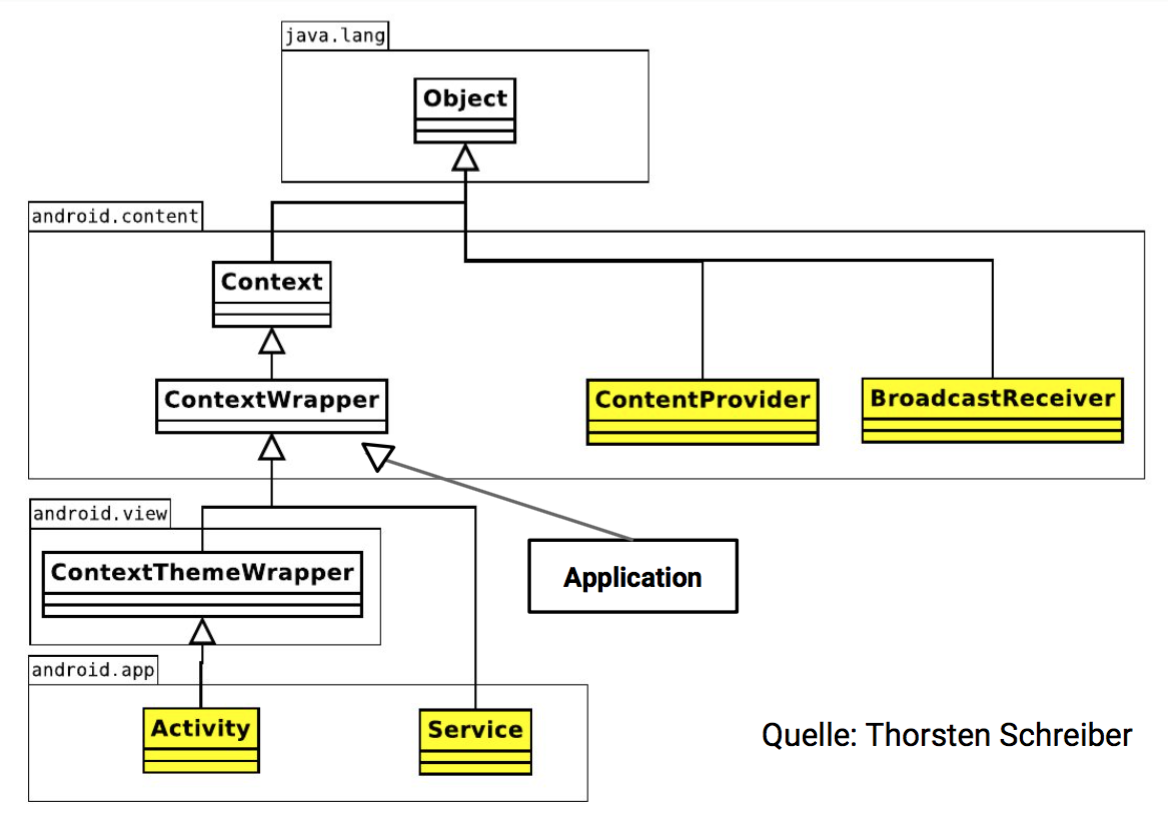
\includegraphics[scale=0.25]{komponentenEinerApp.png}
\paragraph{Context Klasse} Mit einer Context-Instanz kann man:
\begin{itemize}
\item Neue View erstellen (Kontext muss als Parameter mitgegeben werden)
\item Auf System-Service zugreifen (\code{context. getSystemService( LAYOUT\_INFLATER\_SERVICE)})
\item Die Applikationsinstanz erhalten
\item Neue Acativities starten (mittels Intent)
\item Preferences lesen und schreiben
\item Services starten
\end{itemize}
\subsection{Services}
Für Aufgaben die im Hintergrund ablaufen sollen oder deren Abarbeitung das UI zu lange blockieren würde, verwendet man Services (Downloads, Berechnungen, etc.). Services:
\begin{itemize}
\item haben keine Acitivty
\item Können gestarted oder gebunden werden
\item Arbeiten im UI-Thread der Applikation, sind keine eigenen Threads
\item Müssen in der Manifest Datei deklariert werden
\end{itemize}
\paragraph{Services Deklaration} Wie Activities müssen auch Service-Komponenten im Manifest deklariert werden
\begin{lstlisting}[language=java]
<application>
  <service 
  android:name=".ExampleService"
  android:exported="false" />
  <!-- false = Service nur in eigener App -->
</application>
\end{lstlisting}
Es gibt zwei verschiedene Arten von Services. Den \textbf{gebundenen} Service (Client-Server ähnliche Kommunikation über eine längere Zeitdauer) und den \textbf{gestarteten} Service (erledigen einmaliger Aufgaben).
\paragraph{Started Services} Ein Service wird mit \code{context.startService(intent)} gestartet. Der Service läuft im Hintergrund und wird nicht gestoppt, auch wenn der Anwender die App wechselt oder der startende Context zerstört wird (im Hintergrund meint nicht in einem eigenen Thread). Der Service soll sich erst dann selbst beenden, wenn die Arbeit getan ist. Grundsätzlich kann man sagen der Service entkoppelt Aufgaben vom Context, und der AsyncTask entkoppelt Aufgaben vom Main-Thread.
\paragraph{Bound Services} Ein Service wird mit \code{context.bindService(intent, ...)} gebunden. Der Service liefert ein Interface, das dem Client erlaubt, Methoden des Services aufzurufen. Es ist möglich, dass mehrere Clients gebunden sind. Wenn alle Clients \code{context.unbindService(...)} aufgerufen haben, wird der Service zerstört.
Services die immer laufen sollen, auch wenn die App nicht aktiv ist, müssen eine Notification anzeigen.
\paragraph{Lifecycle} Die Callbacks eines Services sind ähnlich wie die der Activitiy
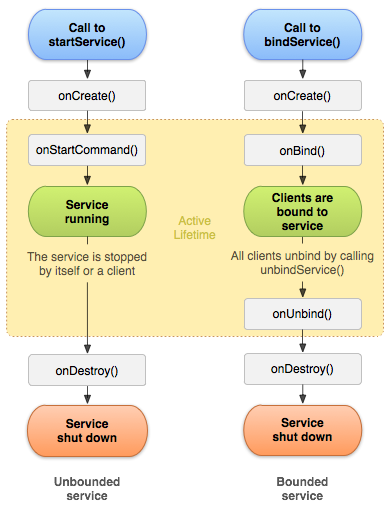
\includegraphics[scale=0.4]{service_lifecycle.png}
\paragraph{Started Service Starten/Stoppen} Der Service wird aus einer Activity gestartet.
\begin{lstlisting}[language=java]
Intent intent = new Intent(this, SimpleService.class);
startService(intent);
\end{lstlisting}
Dies ruft \code{onCreate()} und anschliessen \code{onStartCommand()} im Service auf. Ohne Einstellung, findet keine Kommunikation zwischen Service und Acitivity statt.\\
Der Service kann mit \code{stopSelf()} gestoppt werden und sollte auch getan werden. Man kann den Service auch in der Acitivity stoppen, mittels \code{stopService()}.
\paragraph{Started Service IntentService (Queue)} Der IntentService stellt einen Worker-Thread zur Verfügung. Er verwendet eine Queue, um Intents zwischenzuspeichern, welche sequentiell in \code{onHandleIntent()} abgearbeitet werden. Der Service wird gestoppt, nachdem alle Intents abgearbeitet wurden.
\begin{lstlisting}[language=java]
public class HelloIntentService extends IntentService {
  public HelloIntentService() {
  super("HelloIntentService");
  }
  @Override
  protected void onHandleIntent(Intent intent) { }
}
\end{lstlisting}
\paragraph{Started Service Resultate?}
Wie erhält die Activity ein Resultat vom Services? \code{onHandleIntent()} hat keine Referen auf die aufgerufene Activity. \textbf{Lösung} Service verschickt einen Intent mit Result als Broadcast. Activity stellt Broacast Receiver zur Verfügung, der Intent empfängt
\paragraph{Foreground Services }
Started Services, die für den Benutzer sichtbar sind und nicht vom System unterbrochen werden (z.B Medien abspielen, Statusupdate holen). Vordergrund-Services müssen zwingend eine Notification anzeigen:
\begin{lstlisting}[language=java]
Notification notification = new Notification.Builder(this, CHANNEL_DEFAULT_IMPORTANCE)
                            ...
                            .build();
startForeground(ONGOING_NOTIFICATION_ID, notification); 
\end{lstlisting}

% \paragraph{IntentService vs. AsyncTask}
% Beide blockieren UI nicht. Beim \code{IntentService} ist die Chance höher, dass die Berechnung vollständig durchgeführt wird, da das System Prozesse (APK) mit Services höher gewichtet.

% AsyncTask bietet Callback, IntentService einen Broadcast.

% IntentService zum Wörter zählen (eigentliche Zählmethoden nicht gegeben)
% \begin{lstlisting}[language=java]{language=java}
% @Override
% protected void onHandleIntent(Intent intent) {
%   Log.d(FileActivity.DEBUG_TAG, "onHandleIntent()");

%   // Intent auslesen
%   Bundle bundle = intent.getExtras();
%   if (bundle == null) {
%     Log.d(FileActivity.DEBUG_TAG, "service bundle is null");
%   }

%   FileHolder fileHolder =
%     (FileHolder) bundle.get(FileActivity.KEY_WORD_RESULT);
%   if (fileHolder == null) {
%     Log.d(FileActivity.DEBUG_TAG, "result is null");
%   }

%   // Resultat ermitteln
%   String text = loadFile(fileHolder.id);
%   List<WordCount> counters = analyzeText(text);
%   WordCountResult result = 
%     new WordCountResult(fileHolder, counters);

%   // Activity starten
%   Intent showResultIntent =
%     new Intent(this, WordListActivity.class);
%   Bundle bundle2 = new Bundle();
%   bundle2.putSerializable(FileActivity.KEY_WORD_RESULT, result);
%   showResultIntent.putExtras(bundle2);

%   // Beim starten einer Activity ausserhalb einer Activity
%   // müssen wir dieses Flag setzen:
%   showResultIntent.addFlags(Intent.FLAG_ACTIVITY_NEW_TASK);

%   startActivity(showResultIntent);
% }
% \end{lstlisting}

% Der Service enthält keine Referenz an die aufrufende Activity. Um nun ein Resultat vom Service zu bekommen, kann man entweder einen Intent mit Resultat als Broadcast versenden, wo dann wiederum die Activity einen Broadcast-Receiver zur Verfügung stellen muss um den Intent zu empfangen. Oder man verwendet einen. \code{PendingIntent}.
% \paragraph{Pending Intent} ist ein Objekt das einen Intent umhüllt (wrapped). Genauer ist es ein Token das man einer "{}Fremden App"{} übergiebt (e.g. \code{NotificationManager, AlarmManager} Home Screen \code{AppWidgetManager} oder 3rd Party Apps), welch die "Fremde App" berechtigt bestimmten Code auszuführen. \\
% Wenn man der "{}fremden App"{} einen Intent übergibt, und diese App diesen Intent sendet/broadcastet, dann wird dieser Intent mit seinen eigenen Berechtigungen ausgeführt. Wenn man aber der "fremden App" einen PendingIntent übergibt werden die Berechtigungen der übergebenden App verwendet. Wird die Klasse, welche den PendingIntent erzeugt terminiert, bleibt der PendingIntent bestehen und kann von anderen Apps weiterverwendet werden. Intents behandelen spezifische Komponenten der App, genauso PendingIntents und nutzen dafür z.B. (\code{PendingIntent.getActivity() PendingIntent.getBroadcast() PendingIntent.getService()} \\
% \textbf{Bsp. 1}: Intent erzeugen und wrappen, ausführen der Operation zugehörend zum PendingIntent (\code{send()})
% \begin{lstlisting}[language=java]
% // Explicit intent to wrap
% Intent intent = new Intent(this, LoginActivity.class);

% // Create pending intent and wrap our intent
% PendingIntent pendingIntent = PendingIntent.getActivity(this, 1, intent, PendingIntent.FLAG_CANCEL_CURRENT);
% try {
%   // Perform the operation associated with our pendingIntent
%   pendingIntent.send();
% } catch (PendingIntent.CanceledException e) {
%   e.printStackTrace();
% }
% \end{lstlisting}
% \textbf{Besseres Bsp. 2}: Erzeugen, wrappen, starten mit AlarmManager nach 3 sec.
% \begin{lstlisting}[language=java]
% int seconds = 2;
% // Create an intent that will be wrapped in PendingIntent
% Intent intent = new Intent(this, MyReceiver.class);

% // Create the pending intent and wrap our intent
% PendingIntent pendingIntent = PendingIntent.getBroadcast(this, 1, intent, 0);

% // Get the alarm manager service and schedule it to go off after 3s
% AlarmManager alarmManager = (AlarmManager) getSystemService(ALARM_SERVICE);
% alarmManager.set(AlarmManager.RTC_WAKEUP, System.currentTimeMillis() + (seconds * 1000), pendingIntent);

% Toast.makeText(this, "Alarm set in " + seconds + " seconds", Toast.LENGTH_LONG).show();
% \end{lstlisting}
% Wenn man noch eine BroadcastReceiver onReceive() Methode hinzufügt, vibriert das Gerät für 2 sec. sobald ein Broadcast Event gesendet wurde.
% \begin{lstlisting}[language=java]
% @Override
% public void onReceive(Context context, Intent intent) {
%   // Vibrate for 2 seconds
%   Vibrator vibrator = (Vibrator) context.getSystemService(Context.VIBRATOR_SERVICE);
%   vibrator.vibrate(2000);
% }
% \end{lstlisting}
% \paragraph{Bound Service} Der Bound Service funktioniert nach einem Client-Server Modell. Clients können Methoden eines Service aufrufen und die App kann die Funktionalität des Services andern Apps zur verfügugn stellen. Beim Aufruf von \code{BindService()} erhält der Client ein Interface um mit dem Service zu kommunizieren. Es ist möglich, dass mehrere Clients gleichzeitig gebunden sind. Nachdem alle Clients \code{unbindService()} aufgerufen haben, wird der Service beendet.
% \paragraph{Bound Service: Server} Der Server muss von der Service Klasse und ein Binder implementieren.
% \begin{lstlisting}[language=java]
% public class LocalService extends Service {
%   private final IBinder binder = new LocalBinder();
%   public class LocalBinder extends Binder {
%   LocalService getService() {
%     return LoaclService.this;
%   }
%   }
%   @Override
%   public IBinder onBind(Intent intent) {
%   return binder;
%   }
%   public int getRandomNumber() {
%   return new Random.nextInt(100);
%   }
% }
% \end{lstlisting}
% \paragraph{Bound Service: Client} Ein Bound-Service liefert bei \code{onBind()} ein Interface vom Typ \code{IBinder}. Wenn der Service nur innerhalb der App und im gleichen Prozess arbeitet, sollte ein Binder als Interface geliefert werden. Clients rufen so die Methoden des Binders oder des Services auf.
% \begin{lstlisting}[language=java]
% Intent intent = new Intent(this, LocalService.class);
% bindService(intent, connection, Context.BIND_AUTO_CREATE);
% \end{lstlisting}
% Der Aufruf von \code{bindService()} liefert nicht den \code{onBind()} Binder, sondern der Callback \code{onServiceConnected()} wird aufgerufen.
% \begin{lstlisting}[language=java]
% private ServiceConnection c = new ServiceConnection() {
%   @Override
%   public void onServiceConnected(ComponentName className, IBinder binder) {
%   LocalService.LocalBinder myBinder = (...)binder;
%   LocalService myService = myBinder.getService();
%   int random = myService.getRandomNumer();
%   }
%   @Override
%   public void onServiceDisconeccted(ComponentName name) {}
% };
% \end{lstlisting}
\paragraph{Bound Service} Der Bound Service funktioniert nach einem Client-Server Modell. Clients können Methoden eines Service aufrufen und die App kann die Funktionalität des Services andern Apps zur Verfügung stellen. Beim Aufruf von \code{BindService()} erhält der Client ein Interface um mit dem Service zu kommunizieren. Es ist möglich, dass mehrere Clients gleichzeitig gebunden sind. Nachdem alle Clients \code{unbindService()} aufgerufen haben, wird der Service beendet.

\paragraph{Bound Service: Server} Der Server muss von der Service Klasse und ein Binder implementieren.
\begin{lstlisting}[language=java]
public class LocalService extends Service {
  private final IBinder binder = new LocalBinder();
  public class LocalBinder extends Binder {
  LocalService getService() {
    return LoaclService.this;
  }
  }
  @Override
  public IBinder onBind(Intent intent) {
  return binder;
  }
  public int getRandomNumber() {
  return new Random.nextInt(100);
  }
}
\end{lstlisting}



\paragraph{Bound Service: Client} Ein Bound-Service liefert bei \code{onBind()} ein Interface vom Typ \code{IBinder}.
Der Rückgabewert ist ein Binder.
Wenn der Service nur innerhalb der App und im gleichen Prozess arbeitet, sollte ein Binder als Interface geliefert werden. Clients rufen so die Methoden des Binders oder des Services auf.
\begin{lstlisting}[language=java]
Intent intent = new Intent(this, LocalService.class);
bindService(intent, connection, Context.BIND_AUTO_CREATE);
\end{lstlisting}
Der Aufruf von \code{bindService()} liefert nicht den \code{onBind()} Binder, sondern Callback \code{onServiceConnected()} wird aufgerufen.
\begin{lstlisting}[language=java]
private ServiceConnection c = new ServiceConnection() {
  @Override
  public void onServiceConnected(ComponentName className, IBinder binder) {
  LocalService.LocalBinder myBinder = (...)binder;
  LocalService myService = myBinder.getService();
  int random = myService.getRandomNumer();
  }
  @Override
  public void onServiceDisconeccted(ComponentName name) {}
};
\end{lstlisting}

\paragraph{Bound Service: Messenger} Ein Messenger kann eingesetzt werden um prozessübergreifend Informationen auszutauschen. Der Service stellt dabei einen Handler zur Verfügung um Meldungen zu erhalten, welche er sequentiell abarbeitet. Für Rückgabewerte des Servers muss der Client seinerseits einen Messenger zur Verfügung stellen.


\subsection{Broadcast Receiver} Das System versendet Meldungen per Broadcast. Meldungen werden als Intent verschickt, Action bestimmt Ereignistyp. Eine meldung enthält Informationen über ein bestimmtes Ereignis (SMS empfangen, System wurde gebootet, Akku schwach, etc.) Broadcast Receiver können registriert werden, um bestimmte Meldungen zu erhalten. Apps können auch Meldungen per Broadcast verschicken.

Standardmeldungen des Systems umfassen unter anderem: \code{ACTION\_BOOT\_COMPLETED | ACTION\_POWER\_CONNECTED | ACTION\_POWER\_DISCONNECTED | ACTION\_BATTERY\_LOW | ACTION\_BATTERY\_OKAY}.

\paragraph{Broadcast Receiver: Statisch Registrieren}
Ein Broadcast Receiver wird statisch ins Manifest eingebunden, sodass der Receiver "global" in der App ist:
\begin{lstlisting}[language=java][language=xml]
<receiver android:name=".TimeChangedReceiver" >
  <intent-filter>
  <action android:name="android.intent.action.TIME_SET" />
  </intent-filter>
</receiver>
\end{lstlisting}
\paragraph{Broadcast Receiver: Dynamisch Registrieren}
Wird verwendet, wenn der Receiver an eine Activity gebunden ist, der Receiver muss abgemeldet werden.
\begin{lstlisting}[language=java]
// dynamische Registation in onResume()
LocalBroadcastManager lbm = LocalBroadcastManager.getInstance(getApplicationContext());
IntentFilter filter = new IntentFilter(Intent.ACTION_BOOT_COMPLETED);
MyBroadcastReceiver receiver = new MyBroadcastReceiver(this);
lbm.registerReceiver(receiver, filter);
// Receiver abmelden in onPause()
LocalBroadcastManager lbm = LocalBroadcastManager.getInstance(getApplicationContext());
lbm.unregisterReceiver(receiver);
\end{lstlisting}
\paragraph{Broadcast Receiver: Implementation} Die Implementation eines Receivers muss von der Klasse \code{BroadcastReceiver} ableiten. Die Methode \code{onReceive()} muss überschrieben werden um Meldungen zu erhalten und verarbeiten.
\begin{lstlisting}[language=java]
private class MyBroadcastReceiver extends BroadcastReceiver {
  public MyBroadcastReceiver(MainActivity activity) { }
  @Override
  public void onReceive(Context context, Intent intent){ }
}
\end{lstlisting}
\paragraph{Broadcast Receiver: Versenden} Der Broadcast Receiver kann auch Meldungen versenden. Dies kann man mit der Methode \code{context.sendBroadcast(intent)}. Die Action im angegeben Intent definiert den Ereignistyp (Namensgebend und in der Action ist global, bei eigenen Actions, Name mit eigenem Namespace verwenden). Beim Intent können unter Extras zusätzliche Daten hinterlegt werden. Wenn man Meldungen nur im eigenen selben Prozess versenden möchte, sollte man den \code{LocalBroadcastManger verwenden}. So verlassen die Meldungen den Prozess nicht und andere Prozesse können unserer App keine Meldungen senden.
% \subsection{Content Provider}
% Der Content Provider stellt Daten prozessübergreifend zur Verfügung. Es ist ein Client-Server Modell. Der Provider Client und Provider kommunizieren über eine standartisierte Schnittstelle um Daten auszutauschen. Android stellt beispielsweise Kalender oder Kontakte über einen Content-Provider zur Verfügung.
% \paragraph{Schnittstelle} eines Content Provider stellt in der Regel Daten zur Verfügung die in einer Tabelle in einer Datenbank abgelegt sind. Deshalb ähnelt die Schnittstelle stark der SQL Syntax.\\
% \paragraph{Security} Der Content Provider kann Permissions setzte um den Zugriff auf die Daten einzuschränken. Die Clients müssen die erforderlichen Permissions im Manifest angeben.
% \begin{lstlisting}[language=xml]
% <uses-permission android:name="android.permission.READ_USER_DICTIONARY"/>
% \end{lstlisting}
% \paragraph{Content Provider: Client} Der ContentResolver stellt die Schnittstelle zur Verfügung. Die Tabelle des Content-Provider wird als URI angegeben: \code{content://user\_dictionary/words}.
% \begin{lstlisting}[language=java]
% Cursor cursor = getContentResolver().query(
%   UserDictionary.Words.CONTENT_URI,
%   mProjection,
%   mSelectionClause,
%   mSelectionArgs,
%   mSortOrder);
% int index = cursor.getColumnIndex(UserDictionary.Words.WORD);
% while(cursor.moveToNext()){
%   String word = cursor.getString(index);
% }
% \end{lstlisting}
% \paragraph{Content Provider: Server} Der Einsatz eines eigenen Servers ist erforderlich wenn andere Apps strukturierte Daten oder Dateien zur Verfügung stehen sollen, oder wenn andere Apps die Möglichkeit haben sollen, Daten zu durchsuchen. Ein Provider kann Daten als Dateien oder strukturiert anbieten. Dateien werden im Internal Storage abgelegt, der Client erhält einen Handle um auf eine Datei zuzugreifen. Strukturierte Daten werden in der Regel in einer Datenbank abgelegt. Der ContentResolver hat gezeigt, dass das Prinzip von Tabellen mit Spalten und Reihen verwendet werden sollte. \textbf{Ein Content-Provider muss Thread-Save programmiert werden}.\\
% Bei der Implementation muss man sich folgendes überlegen:
% \begin{itemize}
% \item Wie sollen Daten persistent gespeichert werden
% \item Die Content-URI muss festgelegt werden
% \item Die Klasse \code{ContentProvider} muss implementiert werden.
% \item Eine Contract Klasse muss implementiert werden. Die Klasse enthält alle Bezeichner (Konstanten) die ein Client benötigt. Die Klasse muss zudem in den Applikationscode des Clients kopiert werden.
% \item Permissions in der Manifest Datei müssen festgelegt werden
% \end{itemize}